%
%  untitled
%
%  Created by Stephan Gabler on 2010-05-26.
%  Copyright (c) 2010 __MyCompanyName__. All rights reserved.
%
\documentclass[]{article}

% Use utf-8 encoding for foreign characters
\usepackage[utf8]{inputenc}

% Setup for fullpage use
\usepackage{fullpage}

% Uncomment some of the following if you use the features
%
% Running Headers and footers
%\usepackage{fancyhdr}

% Multipart figures
%\usepackage{subfigure}

% More symbols
%\usepackage{amsmath}
%\usepackage{amssymb}
%\usepackage{latexsym}

% Surround parts of graphics with box
\usepackage{boxedminipage}

% Package for including code in the document
\usepackage{listings}

% If you want to generate a toc for each chapter (use with book)
\usepackage{minitoc}

% This is now the recommended way for checking for PDFLaTeX:
\usepackage{ifpdf}

%\newif\ifpdf
%\ifx\pdfoutput\undefined
%\pdffalse % we are not running PDFLaTeX
%\else
%\pdfoutput=1 % we are running PDFLaTeX
%\pdftrue
%\fi

\ifpdf
\usepackage[pdftex]{graphicx}
\else
\usepackage{graphicx}
\fi
\title{Exercise 4}
\author{Tiziano, Raphael \& Stephan \\ Group n. 2}

\date{\today}

\begin{document}

\ifpdf
\DeclareGraphicsExtensions{.pdf, .jpg, .tif}
\else
\DeclareGraphicsExtensions{.eps, .jpg}
\fi

\maketitle


\section{Task 1: Toy Data PCA}
\begin{figure}[h]
	\centering
		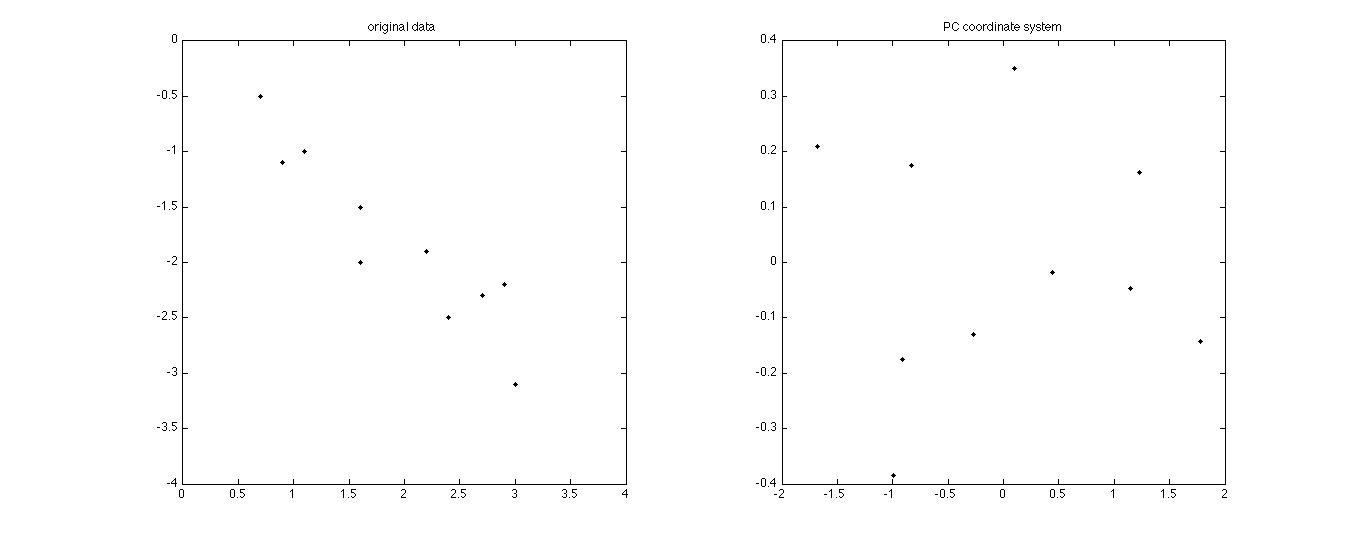
\includegraphics[width=0.6\textwidth]{projection.jpg}
	\caption{Toy data in PCA Space}
	\label{sg:fig:projection}
\end{figure}

\begin{figure}[h]
	\centering
		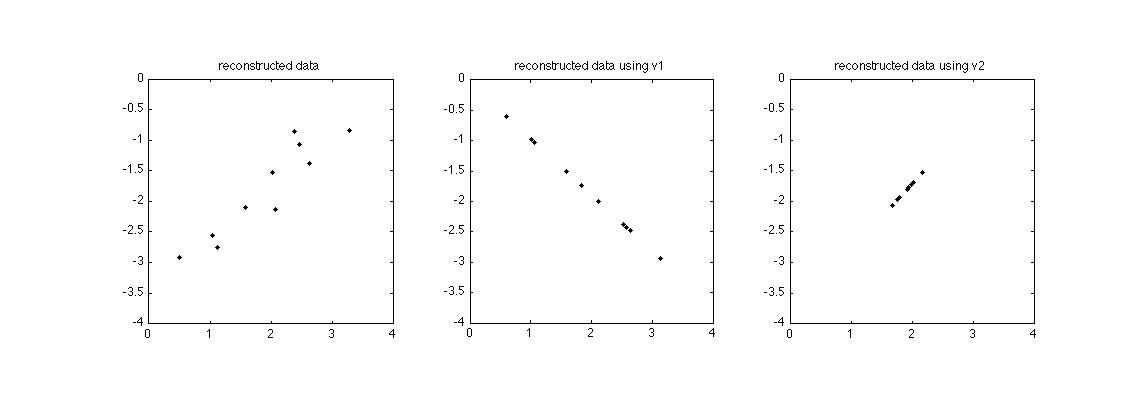
\includegraphics[width=\textwidth]{reconstruction.jpg}
	\caption{Reconstruction of data by using all, one or two PCs}
	\label{sg:fig:reconstruction}
\end{figure}

\section{Image Data} % (fold)
\label{sg:sec:image_data}

\begin{figure}[h]
	\centering
		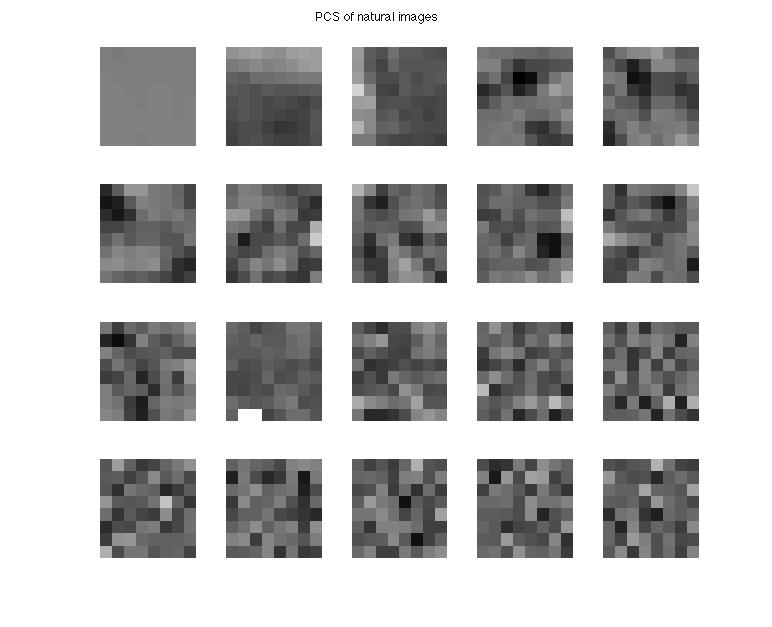
\includegraphics[width=\textwidth]{pc_natural.jpg}
	\caption{PCs of natural images}
	\label{sg:fig:pc_natural}
\end{figure}

\begin{figure}[h]
	\centering
		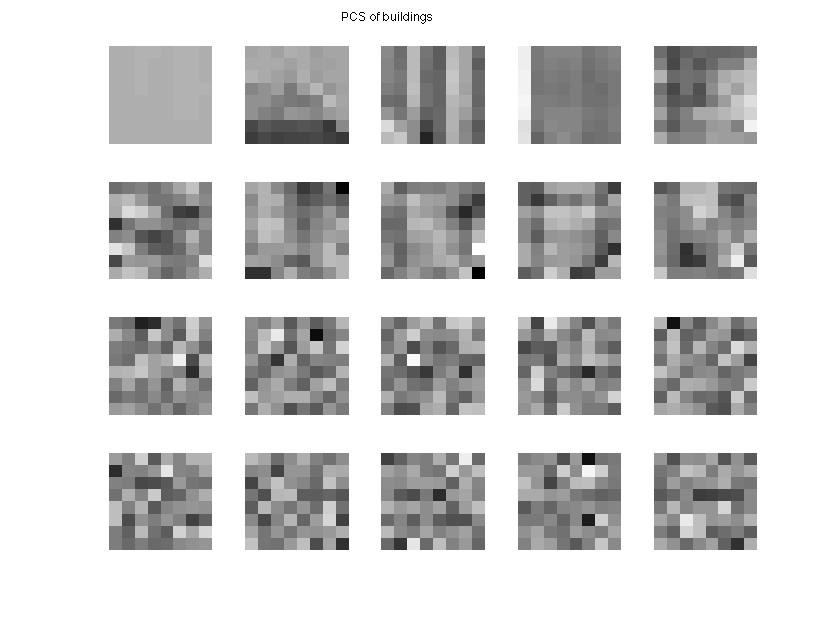
\includegraphics[width=\textwidth]{pc_buildings.jpg}
	\caption{PCs of buildings}
	\label{sg:fig:pc_buildings}
\end{figure}

The principal components of the images of buildings show more rectangular angle orientation.
This is because in the images of buildings there are much more straight and
perpendicular lines.

% section image_data (end)

\clearpage

\section{Kernel PCA} % (fold)
\label{sg:sec:kernel_pca}

The principal components which are lines in the kernel space are gaussians when projected in the input space.
The result also shows that in the kernel space data is linearly separable and this is what we expect because data is also gaussian distributed.
Finally we see that using just the very first principal components we can reconstruct the main structure that is in the data.

\begin{figure}[h]
	\centering
		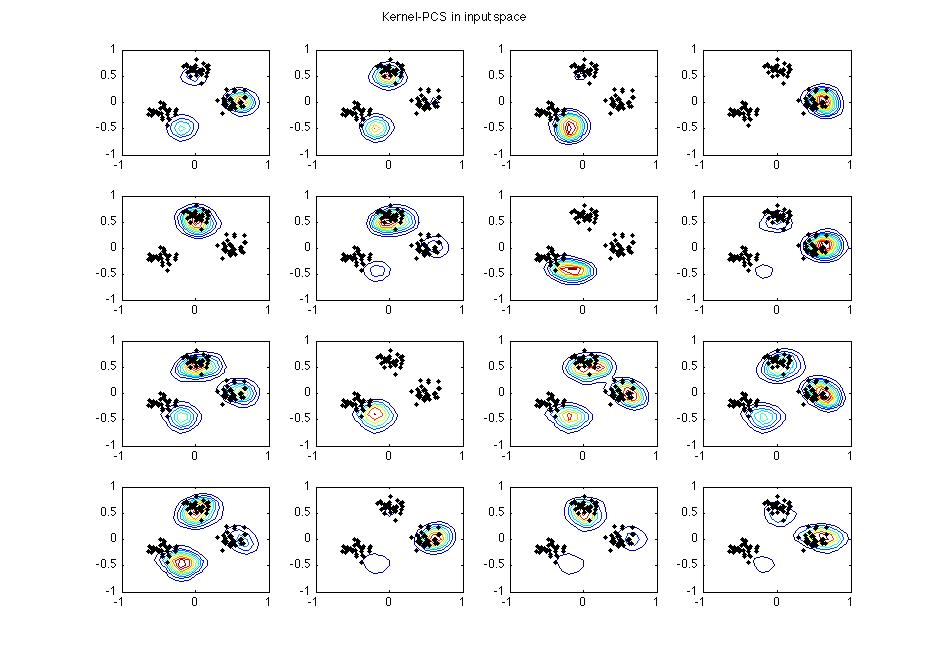
\includegraphics[width=\textwidth]{kernel_pcs.jpg}
	\caption{The Kernel PCs plotted in input space}
	\label{sg:fig:kernel_pcs}
\end{figure}


% section kernel_pca (end)

\end{document}
